\documentclass[a4paper, 12pt]{article}
\usepackage[utf8]{inputenc}
\usepackage[english,russian]{babel}
\usepackage[warn]{mathtext}
\usepackage{graphicx}
\usepackage{float}
\restylefloat{table}
\usepackage{amsmath}
\usepackage{floatflt}
\usepackage[T2A]{fontenc}
\usepackage[left=20mm, top=20mm, right=20mm, bottom=20mm, footskip=10mm]{geometry}

\tolerance 1414
\hbadness 1414
\emergencystretch 1.5em
\hfuzz 0.3pt        % размер максимального переполнения без warning'a
\widowpenalty=10000 % запрещает одиночную строку абзаца в начале страницы
\vfuzz \hfuzz
\raggedbottom       % если на странице мало содержимого, добавить пустое место в конце, а не в середине страницы



\begin{document}

\begin{titlepage}
	\centering
	\vspace{5cm}
	{\scshape\LARGE московский физико-технический институт (национальный исследовательский университет) \par}
	\vspace{6cm}
	{\scshape\Large Лабораторная работа 3.2.5 \par}
	{\huge\bfseries Вынужденные колебания в электрическом контуре \par}
	\vspace{1cm}
	\vfill
\begin{flushright}
	{\large Б03-102}\par
	\vspace{0.3cm}
	{\LARGE Куланов Александр}
\end{flushright}
	

	\vfill


	Долгопрудный, 2022 г.
\end{titlepage}

\begin{itemize}
	\item \textbf{Цель работы:} исследование вынужденных колебаний и процессов их установления в колебательном контуре.
    \item \textbf{В работе используются:} генератор звуковых частот, вольтметр, частотомер, конденсатор, катушка индуктивности, магазин сопротивлений, осциллограф, универсальный измеритель импеданса ($LCR$-метр).
    
\end{itemize}



\section{Теоретические сведения}



\section{Экспериментальная установка}

Схема установки представлена на рисунке \ref{fig:set}. Колебательный контур состоит из конденсатора с ёмкостью
$C$, катушки с индуктивностью $L$ и магазина сопротивлений $R$. Синусоидальный сигнал генерируется звуковым
генератором (ЗГ), а сигнал, состоящий из отрезков синусоиды (цугов), формируется цифровым генератором электрических
сигналов произвольной формы или комбинацией генератора синусоидального сигнала звукового диапазона и электронного 
реле, прерывающего сигнал с заданной периодичностью. Результирующие сигналы --- цуги или непрерывная синусоида 
--- поступают по отдельным каналам через одинаковые небольшие ёмкости $C_1$ соответственно на клеммы "цуги" и "непр."{},
смонтированные на панели "П"{}, на которой расположенны также клеммы "синхр." (синхронизация) и "$\perp$" (земля).
При подключении контура к клемме "$\perp$"{} и через амперметр $A$ к клемме "непр."{} на него подается непрерывный
сигнал --- синусоида; если контур подключен "цуги"{} и "$\perp$"{}, то на контур поступают отрезки синусоиды. 

\begin{figure}[h]
    \centering
    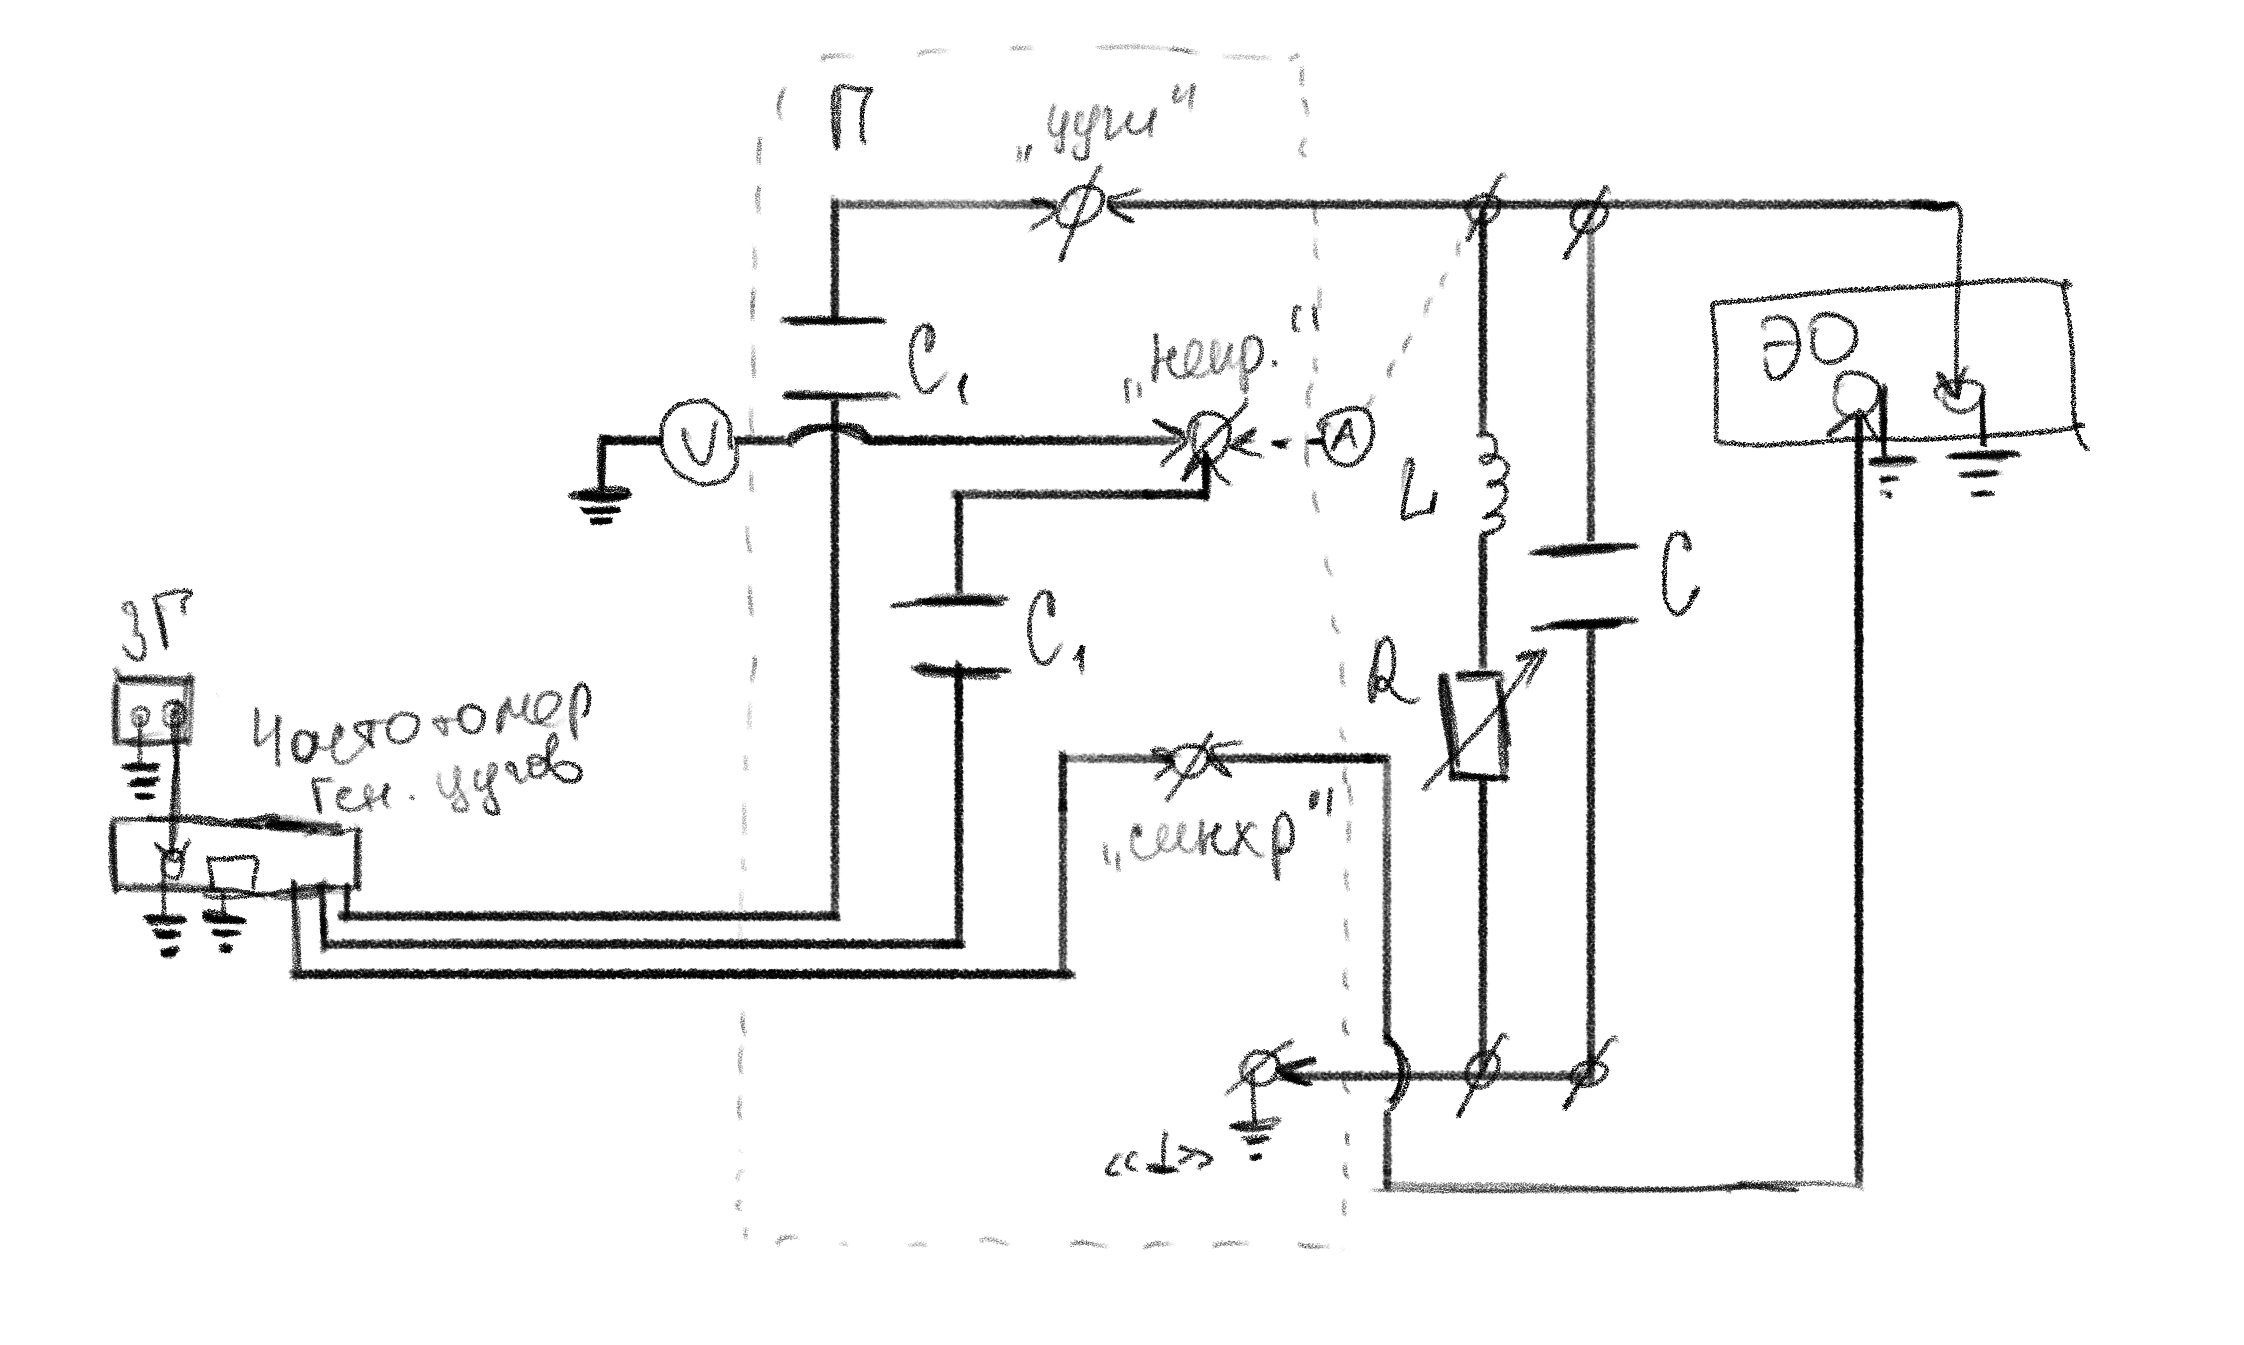
\includegraphics[width=1\textwidth]{set}
    \caption{Схема установки}
    \label{fig:set}
\end{figure}

Эффективное значение тока $I(\omega)$, текущего к контуру от генератора в режиме непрерывного сигнала, 
измеряется амперметром $A$, а соответствующее значение тока в контуре определяется по формуле $I_C(\omega) = \omega C U_C (\omega)$,
где $U_C(\omega)$ --- эффективное напряжение на конденсаторе, измеряемое вольтметром $V$.

Для визуального наблюдения за процессом колебаний напряжение с ёмкости контура $C$ подаётся на вход электронного
осциллографа. Чтобы картина на экране была устойчивой, частота развёртки осциллографа принудительно синхронизируется
с частотой повторения цугов. Для этого на генератор ЭО подаются следующие с частотой повторения цугов управляющие 
импульсы, формируемые в блоке электронного реле, клемма "синхр."{} которого смонтирована на панели "П".

Используя представленную схему в режиме непрерывного синусоидального сигнала, можно по показаниям приборов и известных
параметров элементов цепи измерить амплитудно-частотную характеристику (резонансную кривую) $I_C(\omega)$ в необходимом
диапазоне частот. Сравнивая результат измерения с теоретической кривой, можно определить характеристики контура
$\omega_m \approx \omega_0$ и $Q$.

\section{Обработка результатов}



\section{Приложение}



\end{document}